\documentclass[10pt, conference, compsocconf]{IEEEtran}
\usepackage{graphicx}
\usepackage{float}
\usepackage{amsmath}
\usepackage{hyperref}
\usepackage{booktabs}
\usepackage{booktabs} % For better horizontal rules
\usepackage{siunitx}  % For aligning numbers by decimal point
\hypersetup{
	colorlinks=true,
	linkcolor=black,
	filecolor=magenta,      
	urlcolor=cyan,
}


\title{Structure equation modeling}

\begin{document}
	
	
	\maketitle
	
\section{Overview}	
	\begin{figure}[h!]
		\centering
		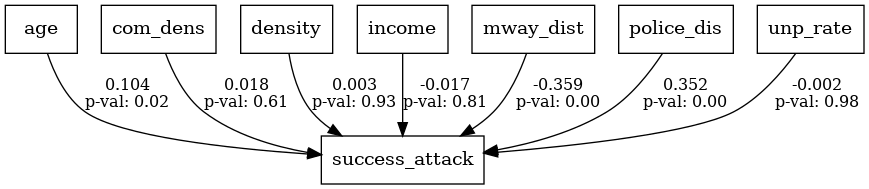
\includegraphics[width=\linewidth]{success.png}
		\caption{SEM Model}
		\label{fig:Model}
	\end{figure}
	
	In Figure \ref{fig:Model}, directional relationship from the predictor variables to the outcome variables is shown. 
	The tilde symbol \textasciitilde,  indicates a directional relationship from the predictor variables to the outcome variable. Essentially, it specifies that success\_attack is regressed on the other variables listed on the right-hand side of the formula.
	
	Name of objective: (ULS) unweighted least square \\
	Optimization method: SLSQP\\
	Objective value: 0.000\\
	Number of iterations: 50
	
\textbf{Equation used}
\begin{subequations}
	\begin{align}
		\begin{split}
			\text{success\_attack} \sim &\, com\_dens + \\
			&\, age + income + \\
			&\, unp\_rate + density + \\
			&\, police\_dis + mway\_dist
		\end{split}
	\end{align}
\end{subequations}

\begin{table}[htbp]
	\centering
	\caption{Parameter Estimates}
	\label{tab:parameter_estimates}
	\begin{tabular}{llSSS}
		\toprule
		Parameter Variable & {Estimate} & {Std. Error} & {z-value} \\
		\midrule
		success\_attack $\longrightarrow$ com\_dens & 0.000337 & 0.000656 & 0.513490 \\
		success\_attack $\longrightarrow$ age & 0.003073 & 0.001354 & 2.270089 \\
		success\_attack $\longrightarrow$ income & -0.000414 & 0.001723 & -0.240056 \\
		success\_attack $\longrightarrow$ unp\_rate & -0.000102 & 0.004123 & -0.024623 \\
		success\_attack $\longrightarrow$ density & 0.000084 & 0.000998 & 0.083945 \\
		success\_attack $\longrightarrow$ police\_dis & 0.000324 & 0.000032 & 10.049766 \\
		success\_attack $\longrightarrow$ mway\_dist & -0.000111 & 0.000014 & -8.217081 \\
		\bottomrule
	\end{tabular}
\end{table}


In Table 1, The values shown helps in assessing the goodness of fit of the model.
The values present in Table 1 convey that the model fits effectively on the dataset. 
In Figure \ref{fig:Model}, it can be observed that no latent variable has been defined which might be the reason for such compatible model.\\
Based on the p\_values of predictor variable we can conclude only age, police and motorway distance are statistically significant. This might be due to because they share a linear relationship with the outcome variable.





	

\end{document}